%
% l2.tex -- L2 Räume 
%
% (c) 2019 Prof Dr Andreas Müller, Hochschule Rapperswil
%
\section{Der Hilbertraum $L^2$
\label{section:l2}}
\rhead{Der Hilbertraum $L^2$}
Bereits im Beispiel auf Seite~\pageref{geometrie:l2-beispiel} wurde
angedeutet, wie man aus einem Funktionenraum einen Hilbertraum
machen kann, indem man ein geeignetes Skalarprodukt definiert.
In diesem Abschnitt soll diese Konstruktion etwas detaillierter 
durchgeführt und verallgemeinert werden.

\subsection{Funktionenräume}
Wir bezeichnen wieder mit $\mathbb C^X$ die Menge der Funktionen
$f\colon X\to \mathbb C$.
Wir haben ihn bereits im Abschnitt~\ref{section:funktionenraume}
zu einem Vektorraum gemacht, indem wir die
Addition von Funktionen und die Multiplikation mit Skalaren
punktweise definiert.
%Seien $f,g$ Funktionen auf $X$, dann definieren wir die Summe $f+g$ und
%$\lambda f$ als
%\begin{align*}
%f+g&\colon X\to\mathbb C: x \mapsto f(x) + g(x)
%\\
%\lambda f &\colon X \to \mathbb C: x \mapsto \lambda f(x).
%\end{align*}

Die Signale, die im Folgenden analysiert werden sollen, sind jedoch
nicht beliebige Funktionen.
Sie haben zusätzliche Eigenschaften, zum Beispiel sind sie oft stetig
oder beschränkt.
Auch den Raum der stetigen Funktionen $C(X,\mathbb C)$ haben wir bereits
in Abschnitt~\ref{section:funktionenraume} zu einem normierten Raum
mit der Supremum-Norm $\|\;\cdot\;\|_\infty$ gemacht.
Wir haben schon damals darauf hingewiesen, dass die Supremum-Norm
nicht von einem Skalarprodukt herkommt und damit nicht harmoniert
mit der Art und Weise, wie wir Funktionen analysieren wollen.

Die Norm als Abstandsbegriff zwischen Funktionen wird zum Zweck der
Approximation durch einfachere Funktionen benötigt.
Die geometrische Intuition erwartet ungefähr die folgenden Eigenschaften
von einem solchen Abstandsbegriff:

\begin{definition}
Eine reellwertige Funktion $\|\mathstrut\cdot\mathstrut\|$ heisst
eine Norm auf dem Vektorraum $V$, wenn sie folgende Eigenschaften hat:
\index{Norm}
\begin{enumerate}
\item $\|v\|=0\;\Leftrightarrow\; v = 0$
\item $\| \lambda u \| = |\lambda| \,\|u\|$
\item $\|u + v\| \le \|u\| + \|v\|$ (Dreiecksungleichung)
\end{enumerate}
\end{definition}

Die Norm, die in Abschnitt~\ref{section:hilbertraum} aus dem Skalarprodukt
gewonnen wurde, hat tatsächlich diese Eigenschaften.
Dabei ist nur die Dreiecksungleichung nicht unmittelbar klar.
Doch aus der Cauchy-Schwarz-Ungleichung folgt
\begin{align*}
\| u + v \|^2
&=
\langle u+v,u+v\rangle
=
\| u \|^2 + 2\operatorname{Re} \langle u,v\rangle + \| v\|^2
\\
&\le
\| u \|^2 + 2|\operatorname{Re} \langle u,v\rangle| + \| v\|^2
\\
&\le
\| u \|^2 + 2|\langle u,v\rangle| + \| v\|^2
\\
&\le
\| u \|^2 + 2\| u \| \cdot \|v\| + \| v\|^2
=
(\|u\| + \| v \|)^2
\\
\Rightarrow\qquad\qquad
\|u+v\|
&\le
\|u\| + \|v\|.
\end{align*}

Unser nächstes Ziel muss daher sein, auf den Funktionenräumen ein
Skalarprodukt zu definieren.
Daraus ergibt sich dann automatisch eine für unsere Zwecke geeignete
Norm.

%\begin{definition}
%Der Vektorraum der stetigen Funktionen auf $X\subset R^n$ ist die Menge
%\[
%C_{\mathbb C}(X)
%=
%C(X)
%=
%\{ f\in \mathbb C^X\,|\, \text{$f$ ist stetig}\}
%\]
%mit der punktweisen Addition und Multiplikation mit Skalaren und der
%Norm
%\[
%\| f \| = \sup_{x\in X} |f(x)|.
%\]
%$\|f\|$ heisst auch die Supremum-Norm.
%\end{definition}

%Man beachte, dass diese Norm nicht von einem Skalarprodukt herkommt.
%Man kann aber zeigen, dass Cauchy-Folgen in dieser Norm gegen eine
%stetige Funktion konvergieren.
%Diese Norm stellt also sicher, dass die Grenzfunktion einer
%Approximationsfolge aus stetigen Funktion wieder stetig ist.
%Umgekehrt können wir bei einer anderen Norm wie der im nächsten
%Abschnitt definierten $L^2$-Norm nicht mehr garantieren, dass 
%Grenzfunktionen stetig sind.
%Dies verursacht zwar ein paar mathematische Unannehmlichkeiten,
%kommt aber den Anwendungen entgegen, da in der Praxis durchaus
%nicht stetige Signale vorkommen.

\subsection{Definition des Skalarproduktes}
In diesem Abschnitt betrachten wir ausschliesslich komplexwertige Funktionen,
die auf einem endlichen oder unendlichen Interval $I$ definiert sind.

\begin{definition}
\label{l2:definition:skalarprodukt}
\index{Skalarprodukt in $L^2$}%
Das Skalarprodukt zweier Funktionen $f,g\colon I\to\mathbb C$ ist definiert
als
\begin{equation}
\langle f,g\rangle
=
\int_I f(t) \bar{g}(t)\,dt.
\label{l2:formel:skalarprodukt}
\end{equation}
\end{definition}

Die bekannten Rechenregeln für Integrale stellen sicher, dass dies
tatsächlich ein sesquilineares Produkt ist, wie die folgende Rechnung
zeigt:
\begin{align*}
\langle \lambda_1 f_1+\lambda_2 f_2,g\rangle
&=
\int_I (\lambda_1 f_1(t) + \lambda_2 f_2(t))\bar{g}(t)\,dt
\\
&=
\lambda_1 \int_I f_1(t) \bar{g}(t)\,dt + \lambda_2 \int_I f_2(t)\bar{g}(t)\,dt
= \lambda_1 \langle f_1,g\rangle + \lambda_2 \langle f_2,g\rangle
\\
\langle f,\mu_1 g_1 + \mu_2 g_2\rangle
&=
\int_I f(t) \overline{(\mu_1 g_1(t) + \mu_2 g_2(t))}\,dt
=
\bar{\mu}_1 \int_I f(t) \bar{g}_1(t)\,dt
+
\bar{\mu}_2 \int_I f(t) \bar{g}_2(t)\,dt
\\
&=
\bar{\mu}_1 \langle f,g_1\rangle
+
\bar{\mu}_2 \langle f,g_2\rangle
\\
\overline{
\langle f,g\rangle
}
&=
\overline{ \int_I f(t)\bar{g}(t)\,dt}
=
\int_i \bar{f}(t) g(t)\,dt
=
\int_i g(t) \bar{f}(t)\,dt
=
\langle g,f\rangle.
\end{align*}
Die algebraischen Eigenschaften eines komplexen Skalarproduktes sind
also erfüllt.

\subsubsection{Unstetige Grenzfunktionen}
\begin{figure}
\centering
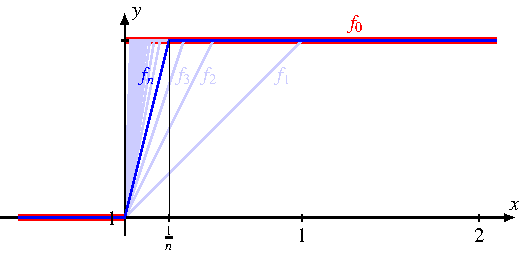
\includegraphics{chapters/2-fourier/images/lim.pdf}
\caption{Der Grenzwert $f_0$ einer Folge von stetigen Funktionen $f_n$
braucht nicht stetig zu sein.
\label{fourier:grenzwertunstetig}}
\end{figure}
Die aus \eqref{l2:formel:skalarprodukt} abgeleitete Norm überrascht uns
damit, dass Grenzfunktionen einer Folge stetiger Funktionen nicht mehr
stetig sein müssen.
Wir betrachten dazu das folgende Beispiel.

\begin{beispiel}
Die Funktionen
\[
f_n(t)
=
\begin{cases}
0&\qquad t\le 0\\
nt&0<t\le \frac1n\\
1&\qquad t\ge 0
\end{cases}
\]
sind für alle $n>1$ stetig (siehe auch
Abbildung~\ref{section:funktionenraume}).
Die Funktion
\[
f_0(t) = \begin{cases}
0&\qquad t \le 0\\
1&\qquad t>0
\end{cases}
\]
ist dagegen unstetig.
Die Funktionen $f_n$ und $f_0$ unterscheiden sich nur in einem Interval
der Länge $\frac1n$, der Unterschied ist $\le 1$.
Damit können wir den Unterschied in der Norm berechnen:
\[
\| f_n - f_0 \|^2
=
\int_{-\infty}^{\infty}
|f_n(t)-f_0(t)|^2
\,dt
\le
\int_0^{\frac1n} 1\,dt
=
\frac1n.
\]
Wir schliessen daher, dass $f_n$ im Sinne der Norm gegen $f_0$ konvergiert.
Die Grenzfunktion $f_0$ ist aber nicht stetig.
\end{beispiel}

Das Beispiel zeigt, dass der Funktionenraum der stetigen Funktionen nicht
der geeignete Rahmen für eine Hilbertraum-Theorie für Signale sein kann.
Andererseits kommt dies der Anwendung sehr entgegen, in denen unstetige
Signale wie Rechteck- oder Sägezahn-Signale von grosser praktischer
Bedeutung sind.
Im Folgenden muss daher geklärt werden, welche Art von Funktionen überhaupt
verwendet werden soll.

\subsubsection{Nullmengen und Nullfunktionen}
Es ist bis jetzt nicht klar, ob das Produkt~\eqref{l2:formel:skalarprodukt}
auch tatsächlich definit ist.
Dazu betrachten wir die aus dem Skalarprodukt abgeleitete Norm
\[
\|f\|^2 = \int_I |f(t)|^2\,dt \ge 0.
\]
Für eine stetige Funktion gilt sicher, dass die Norm nur dann verschwinden
kann, wenn der Integrand überall $=0$ ist.
Allerdings wissen wir auch, dass wir uns nicht auf stetige Funktionen
beschränken dürfen.

Eine Funktion, die nur an endlich vielen Stellen nicht verschwindet,
ist immer noch integrierbar und ihr Integral ist $0$.
Eine solche Funktion hätte also Norm $0$ ohne überall $=0$ zu sein.
Zwei Funktionen, die sich um eine solche Funktion unterschieden, 
sind mit der Norm nicht unterscheidbar.

Dies deutet an, dass wir bei der Auswahl der Funktionenmenge, mit der
wir arbeiten wollen, sehr viel sorgfältiger sein müssen.
Doch auch der Begriff des Integrals erfordert einer Revision.
Das Riemann-Integral, das man im Analysis-Unterricht kennen lernt, 
ist leider nicht geeignet für das vorliegende Approximationsproblem.
Eine Funktion soll durch quadratintegrierbare Funktionen approximiert
werden im Sinne der Norm $\|\mathstrut\cdot\mathstrut\|_2$.
Doch kann man leicht Folgen konstruieren, die im Sinne dieser Norm
Cauchy-Folgen sind, aber die Grenzfunktion ist nicht mehr integrierbar.

\begin{beispiel}
Die Menge $[0,1]\cap \mathbb Q$ der rationalen Zahlen im Interval
$[0,1]$ ist abzählbar, es gibt  also eine Folge $q_k$, die alle rationalen
Zahlen durchläuft.
Daraus kann man jetzt eine Funktionen-Folge $f_n$ wie folgt konstruieren:
\[
f_n(t) = \begin{cases} 
1&\qquad \text{$t=t_k$ für ein $k\le n$}\\
0&\qquad\text{sonst}.
\end{cases}
\]
Jede der Funktionen $f_n$ ist integrierbar, denn sie weichen nur an
endlich vielen, genauer an $n$ Stellen von $0$ ab.
Ihr Integral ist daher $0$.
Der Abstand zwischen zwei Funktionen der Folge ist $\| f_n-f_m\|_2 = 0$,
da auch die Differenz nur an endlich vielen Stellen von $0$ verschieden ist.
Trotzdem kann man nicht sagen, dass die Folge eine Grenzfunktion hat.
Punktweise konvergiert die Folge $f_n$ gegen die Funktion
\[
f_{\mathbb Q}(t) = \begin{cases}
1&\qquad t\in\mathbb Q\\
0&\qquad\text{sonst}
\end{cases}
\]
Diese Funktion ist aber nicht einmal integrierbar im Sinne des
Riemann-Integrals.
\end{beispiel}

Die Funktion $f_{\mathbb{Q}}$ ist in jedem Punkt des Definitionsbereichs
unstetig, aber sie ist der Grenzwert einer Folge von Funktionen, die
alle Riemann-integrierbar sind und Integral $0$ haben.
Das Riemann-Integral verträgt sich nicht gut mit Grenzwertbildung.

Die intuitive Vorstellung des ``Volumens'' der Menge 
$[0,1]\cap\mathbb{Q}$ zeigt, dass das Problem tiefer liegt.
Die Menge $[0,1]\cap\mathbb{Q}$ ist abzählbare Vereinigung von Mengen $\{q_n\}$,
die natürlich alle Volumen $0$ haben.
Trotzdem liegt die Menge $[0,1]\cap\mathbb{Q}$ dicht im Interval $[0,1]$,
die geometrische Intuition möchte ihr daher das Volumn $1$ geben.

\subsubsection{Lebesgue-Integral}
\index{Lebesgue-Integral}%
\index{Lebesgue, Henri}%
Die Lösung besteht darin, den Integralbegriff zu erweitern.
Dies ist Henri Lebesgue in seiner Dissertation 1902 gelungen.
Das Lebesgue-Integral ist für alle Riemann-integrierbaren Funktionen
definiert und ergibt denselben Wert.
Die bekannten Berechnungsregeln für Integrale bleiben daher erhalten
und Algorithmen zur numerischen Berechnung von Integralen haben
weiterhin ihre Gültigkeit.

Das Lebesgue-Integral erweitert die Menge der integrierbaren Funktionen
und stellt insbesondere sicher, dass die Grenzfunktionen von Folgen
unter genügend allgemeinen Voraussetzungen integrierbar sind und dass
Integral und Grenzwert vertauschbar sind.
Damit ist die Klasse gross genug für das Approximationsproblem.

Abzählbare Mengen wie $\mathbb Q$ haben kein Lebesgue-Mass, sie
gelten als Mengen mit Mass Null oder {\em Nullmengen}.
\index{Nullmenge}%
Für das Riemann-Integral sind nur die endlichen Mengen Nullmengen,
das Lebesgue-Integral erweitert die Klasse der Nullmengen soweit,
dass abzählbare Vereinigungen von Nullmengen immer auch wieder
Nullmengen sind.

Das Lebesgue-Integral betrachtet die Funktion $f_{\mathbb Q}$ 
als integrierbar mit Integralwert $0$.
Allgemein heisst eine Funktion, die überall ausser auf einer Nullmenge
verschwindet, eine {\em Nullfunktion}.
Man sagt auch, die Funktion sei {\em fast überall} $0$.
\index{Nullfunktion}
Das Integral einer beliebigen Nullfunktion ist $0$.

Für eine beliebige integrierbare Funktion $g$ ist daher auch 
$g+f_{\mathbb Q}$ integrierbar und hat den gleichen Integralwert
wie $g$.
Dies gilt auch für jede andere Nullfunktion an Stelle von $f_{\mathbb Q}$.
Man sagt, zwei Funktionen seien {\em fast überall} gleich, wenn sie sich
nur um eine Nullfunktion unterscheiden.
\index{fast überall}%
In $\mathcal{L}^p$ sind daher sehr viele Funktionen nicht unterscheidbar,
da sie sich nur um eine Nullfunktion unterscheiden.

\begin{definition}
\index{$L^p(I)$}%
Die Menge $L^p(I)$ besteht aus Äquivalenzklassen von Funktionen in
$\mathcal{L}^p(I)$, die sich durch eine Nullfunktion unterscheiden.
Zwei Funktionen $f_1,f_2\in L^p(I)$ werden als gleich betrachtet,
wenn
\[
\int_I
|f_2-f_1|
\,dx
=0
\]
ist.
\end{definition}

Die Menge $L^p(I)$ erbt von $\mathcal{L}^p(I)$ die Struktur eines
Vektorraums mit der Norm $\|\mathstrut\cdot\mathstrut\|_p$.
Der Raum $L^2(I)$ wird dank der oben formulierten Grenzwertsätze zu
einem Hilbertraum.
Damit ist der Raum $L^2(I)$ als die Bühne für die nachfolgend zu diskutierende
Approximationstheorie bereitgestellt.

Die Definition von $L^p(I)$ als Menge von Äquivalenzklassen von Funktionen
ist etwas schwerfällig und ungewohnt, für die Praxis aber kaum von Bedeutung.
Jegliche Rechnungen mit Funktionen finden immer mit einem
Riemann-integrierbaren Repräsentaten statt.


Die Definition ist natürlich nur sinnvoll für Funktionen, für die diese
Integrale tatsächlich existieren.
\begin{definition}
Sei $p\in \{1,2\}$ 
\begin{align*}
\mathcal{L}^p(I)
=
\left\{ f \in \mathbb C^I \, \left|
\text{
$f$ ist integrierbar und $\int_I |f(t)|^p\,dt<\infty$
}
\right.\right\}
\end{align*}
mit zugehöriger Norm
\[
\|f\|_p = \biggl(\int_I |f(t)|^p \,dt\biggr)^{\frac1p}.
\]
\end{definition}

Für $p=2$ ist die Norm $\|f\|_2$ bereits bekannt, es ist die Norm, die
vom Skalarprodukt herkommt.

\subsubsection{Beziehung zwischen $\mathcal{L}^1(I)$ und $\mathcal{L}^2(I)$}
Die Beziehung der Funktionenräume $\mathcal{L}^1(I)$ und $\mathcal{L}^2(I)$
zueinander ist nicht ganz offensichtlich.
Die folgenden Beispiele sollen zeigen, dass der Definitionsbereich
dabei eine wichtige Rolle spielt.
Wir beginnen damit zu zeigen, dass auf einem beschränkten Interval
die quadratintegrierbaren Funktionen eine echte Teilmenge der integrierbaren
Funktionen bilden.

\begin{lemma}
\label{fourier:l1l2}
Ist $I$ ein beschränktes Interval, dann ist $\mathcal{L}^2(I)$ eine
echte Teilmenge von $\mathcal{L}^1(I)$.
Es gibt also eine integrierbare Funktion auf $I$, die nicht
quadratintegrierbar ist.
\end{lemma}

\begin{proof}[Beweis]
\begin{figure}
\centering
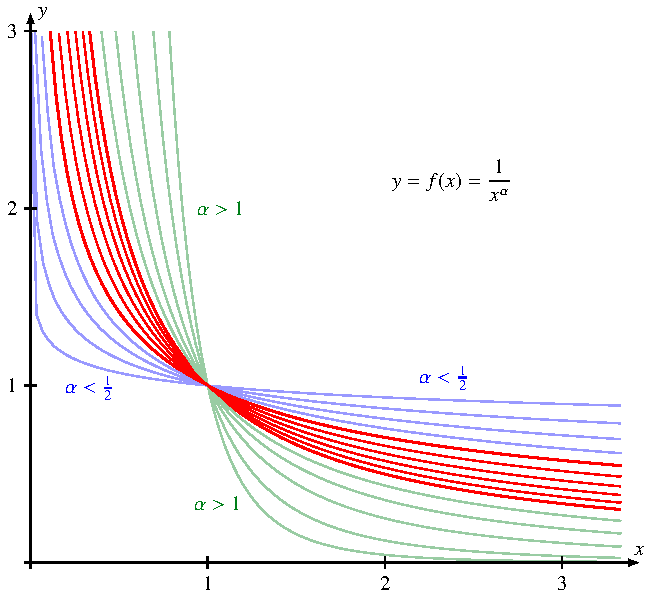
\includegraphics{chapters/2-fourier/images/intfun.pdf}
\caption{Funktionen der Form $f(x)=x^{-\alpha}$ auf dem Interval
$[0,\frac{10}{3}]$ sind nicht integrierbar für $\alpha > 1$ (grün).
Für $\alpha <\frac12$ ist $f(x)$ quadratintegrierbar und auch integrierbar.
Dazwischen, für $\frac12 <\alpha < 1$, ist $f(x)$ zwar integrierbar, aber
nicht quadratintegrierbar.
\label{fourier:intfun}}
\end{figure}
Sei $f\in\mathcal{L}^2(I)$, es gilt also
\[
\int_I |f(x)|^2\,dx < \infty.
\]
Wir versuchen jetzt, dass Integral von $|f(x)|$ zu berechnen.
Dazu verwenden wir, dass wir $|f(x)|$ als das Produkt
$|f(x)|\cdot 1$ mit der Konstanten Funktion $1$ schreiben
und die Cauchy-Schwarz-Ungleichung auf das Produkt anwenden können:
\begin{align*}
%\|f\|_1
%&
%=
\int_I |f(x)|\,dx
&=
\int_I |f(x)| \cdot 1 \,dx
=
\langle |f|, 1\rangle
\le
\|f\|_2 \cdot \| 1 \|_2
\\
&=
\int_I |f(x)|^2\,dx \cdot \int_I 1\,dx
\end{align*}
Da das Interval $I$ beschränkt ist, ist das rechte Integral gerade die
Länge des Intervals.
Das erste Integral ist die Norm $\|f\|_2$, so dass wir ablesen können,
dass $\|f\|_1$ beschränkt ist.
Eine quadratintegrierbare Funktion ist also automatisch integrierbar,
$\mathcal{L}^2(I)\subset \mathcal{L}^1(I)$.

Um zu zeigen, dass $\mathcal{L}^2(I)$ eine echte Teilmenge von 
$\mathcal{L}^1(I)$ ist, 
müssen wir jetzt eine integrierbare Funktion
finden, die nicht quadratintegrierbar ist.
Wir nehmen dazu an, dass $I=[a,b]$ und versuchen eine Funktion der Form
\begin{align*}
f(x)
&=
\begin{cases}
0&\qquad x=a\\
(x-a)^\alpha&\qquad x>a.
\end{cases}
\end{align*}
Die Norm für $p=1$ ist
\begin{align*}
\|f\|_1
&=
\int_a^b |f(x)|\,dx
=
\int_a^b (x-a)^\alpha\,dx 
=
\int_0^{b-a} \xi^\alpha\,d\xi
=
\biggl[
\frac{1}{\alpha+1}\xi^{\alpha+1}
\biggr]_0^{b-a}
\intertext{mit der Substition $x=a+\xi$.
Für $p=2$ kann man die gleiche Formel mit $2\alpha$ an Stelle
von $\alpha$ vewenden:}
\|f\|_2^2
&=
\biggl[
\frac{1}{2\alpha+1}\xi^{2\alpha+1}
\biggr]_0^{b-a}.
\end{align*}
Das Integral existiert also genau dann, wenn der Exponent von $\xi$
positiv ist.
Wenn $\alpha$ so gewählt wird, dass $\alpha+1>0$ und $2\alpha+1 <0$ ist,
dann haben wir ein Beispiel der gesuchten Art gefunden.
Die beiden Ungleichungen bedeuten $\alpha >-1$ und $\alpha < -\frac12$.
Die Funktionen
\[
f_\alpha(x)
=
\begin{cases}
\displaystyle\frac{1}{(x-a)^\alpha}&\qquad x > a\\
0&\qquad x=a
\end{cases}
\]
sind für
$\frac12 <\alpha < 1$
integrierbar, aber nicht quadratintegrierbar.
Die Funktionen $f_\alpha(x)$ sind in Abbildung~\ref{fourier:intfun}
dargestellt.
\end{proof}

Das nachfolgende Beispiel sollen zeigen, dass die Situation für eine
unbeschränktes Interval viel komplizierter ist.
Insbesondere gibt es quadratintegrierbare Funktionen auf $\mathbb R$,
die nicht integrierbar sind, und integrierbare Funktionen, die nicht
quadratintegrierbar sind.

\begin{beispiel}
Den Funktion $f_\alpha$, die in Beweis von Lemma~\ref{fourier:l1l2}
verwendet wurden, haben ausgenutzt, dass sie für $x\to 0$ verschieden 
schnell divergiert haben.
Das Verhalten für $x\to \frac{10}3$ war nicht relevant, weil dort keine
Divergenz auftrat.

Auf dem unbeschränkten Interval $I=[0,\infty)$ kann eine Funktion 
für $x\to\infty$ zwar gegen Null gehen, aber das Integral kann trotzdenm
divergieren.
Diese Eigenschaft können wir ausnützen, um zu zeigen, dass weder
$\mathcal{L}^1(I)\subset\mathcal{L}^2(I)$
noch
$\mathcal{L}^2(I)\subset\mathcal{L}^1(I)$.

Wir betrachten zunächst die Funktionen
\[
f_\alpha(x) = \begin{cases}
\displaystyle\frac1{x^\alpha}&\qquad0<x\le 1\\
0&\qquad\text{sonst.}
\end{cases}
\]
Gemäss der früheren Rechnungen ist
$f_\alpha\in\mathcal{L}^1(I)\setminus\mathcal{L}^2(I)$,
wenn $\frac12<\alpha<1$.

Andererseits können wir auch die Funktionen
\[
g_\beta(x)
=
\begin{cases}
\displaystyle\frac1{x^\beta}&\qquad x>1\\
0&\qquad\text{sonst}
\end{cases}
\]
betrachten.
Wir berechnen wieder die Normen
\begin{align*}
\| g_\beta\|_1
&=
\int_I|g_\beta(x)|\,dx
=
\int_1^\infty x^{-\beta}\,dx
=
\biggl[
\frac1{-\beta+1}x^{-\beta+1}
\biggr]_1^\infty
\\
\|g_\beta\|_2^2
&=
\biggl[
\frac1{-2\beta+1}x^{-2\beta+1}
\biggr]_1^\infty
\end{align*}
Die Normen existieren genau dann, wenn die Exponenten negativ sind.
Die Norm für $p=1$ ist also beschränkt, wenn $-\beta+1<0$ oder $\beta > 1$
ist.
Die Norm für $p=2$ ist beschränkt, wenn $-2\beta+1<0$ oder $\beta > \frac12$
ist.
Für $\beta$ zwischen $\frac12$ und $1$ ist $g_\beta$ also quadratintegrierbar
aber nicht integrierbar.
Somit ist $g_\beta\in\mathcal{L}^2(I)\setminus\mathcal{L}^1(I)$.
Die beiden Beispiele zeigen, dass weder
$\mathcal{L}^1(I)\subset\mathcal{L}^2(I)$
noch
$\mathcal{L}^2(I)\subset\mathcal{L}^1(I)$.
\end{beispiel}

\subsubsection{Vollständigkeit}
Das Lebesgue-Integral wurde sorgfältig so konstruiert, dass Grenzfunktionen
von Funktionenfolgen unter sehr milden Voraussetzungen als Integral den
Grenzwert der Integrale der Folgenglieder haben.
Genauer gilt der folgende grundlegende Satz.

\begin{satz}[Lebesgue]
\label{satz:domkonv}
Ist $f_n$ eine Folge integrierbarer Funktionen, die durch eine
integrierbare Funktion $g$ beschränkt ist:
$
|f_n| \le |g|
$
für alle $n$, dann gibt es eine integrierbare Funktion $f$, so dass
$f_n$ fast überall gegen die Funktion $f$ konvergiert und es gilt
\[
\lim_{n\to\infty} \int_I f_n(x)\,dx = \int_I f(x)\,dx.
\]
\end{satz}

Die Grenzfunktion $f$ ist nicht eindeutig. 
Jede andere Funktion, die sich nur auf einer Nullmenge von $f$ unterscheidet,
kommt genauso als Grenzfunktion in Frage.
Die Grenzfunktion ist daher eigentlich eine Äquivalenzklasse in $L^1(I)$.
Wir sollten daher den Satz~\ref{satz:domkonv}
besser für $L^1(I)$ formulieren.

\begin{satz}
\label{satz:domkonv}
Ist $f_n\in L^1(I)$ durch $g\in L^1(I)$ beschränkt, also $|f_n|\le |g|$,
dann ist $\lim_{n\to\infty}f_n\in L^1(I)$ und es gilt
\[
\lim_{n\to\infty} \int_I f_n(x)\,dx = \int_I \lim_{n\to\infty} f_n(x)\,dx.
\]
\end{satz}

Auch andere aus der Theorie des Riemann-Integrals bekannte Formeln gelten
weiterhin, zum Beispiel die Formel
\[
\int_a^b \int_c^d f(x,y) \,dx \,dy
=
\int_c^d
\int_a^b
f(x,y)
\,dy
\,dx,
\]
die auch als {\em Satz von Fubini} bekannt ist.
\index{Fubini, Satz von}%
Die Reihenfolge von Integrationen kann also unter gewissen
technischen Bedingungen vertauscht werden.

Die Vektorräume $L^1(I)$ und $L^2(I)$ haben daher genau die Eigenschaften,
die wir brauchen.
Man kann darin beliebige Grenzwerte bilden und die Grenzwerte verhalten
sich so, dass man den Grenzübergang aus dem Integral herausziehen kann.
Die gewohnten Formeln aus der Theorie des Riemann-Integrals sind weiterhin
anwendbar, die dort gewonnene Intuition bleibt zuverlässig.
Die gesamte zu entwickelnde Theorie wird sich daher in diesen Räumen
abspielen.
Die etwas unintuitive Definition als Menge von Äquilvalenzklassen hat
keine praktische Konsequenzen, da für stetige oder stückweise stetige
Funktionen das Lebesgue-Integral mit dem Riemann-Integral übereinstimmt.
Für Funktionen von praktischer Relevanz sind daher die bekannten
Integrationstechniken anwendbar.

%\subsection{Lebesgue-Integral und Vollständigkeit}
%Das Riemann-Integral, das man im Analysis-Unterricht kennen lernt, 
%ist leider nicht geeignet für das vorliegende Approximationsproblem.
%Eine Funktion soll durch quadratintegrierbare Funktionen approximiert
%werden im Sinne der Norm $\|\mathstrut\cdot\mathstrut\|_2$.
%Doch kann man leicht Folgen konstruieren, die im Sinne dieser Norm
%Cauchy-Folgen sind, aber die Grenzfunktion ist nicht mehr integrierbar.

%\begin{beispiel}
%Die Menge $[0,1]\cap \mathbb Q$ der rationalen Zahlen im Interval
%$[0,1]$ ist abzählbar, es gibt  also eine Folge $q_k$, die alle rationalen
%Zahlen durchläuft.
%Daraus kann man jetzt eine Funktionen-Folge $f_n$ wie folgt konstruieren:
%\[
%f_n(t) = \begin{cases} 
%1&\qquad \text{$t=t_k$ für ein $k\le n$}\\
%0&\qquad\text{sonst}.
%\end{cases}
%\]
%Jede der Funktionen $f_n$ ist integrierbar, denn sie weichen nur an
%endlich vielen, genauer an $n$ Stellen von $0$ ab.
%Ihr Integral ist daher $0$.
%Der Abstand zwischen zwei Funktionen der Folge ist $\| f_n-f_m\|_2 = 0$,
%da auch die Differenz nur an endlich vielen Stellen von $0$ verschieden ist.
%Trotzdem kann man nicht sagen, dass die Folge eine Grenzfunktion hat.
%Punktweise konvergiert die Folge $f_n$ gegen die Funktion
%\[
%f_{\mathbb Q}(t) = \begin{cases}
%1&\qquad t\in\mathbb Q\\
%0&\qquad\text{sonst}
%\end{cases}
%\]
%Diese Funktion ist aber nicht einmal integrierbar im Sinne des
%Riemann-Integrals.
%\end{beispiel}

%Das Beispiel illustriert die Unzulänglichkeit des Riemann-Integrals.
%Die Lösung besteht darin, den Integralbegriff zu erweitern.
%Dies ist Henri Lebesgue in seiner Disseration 1902 gelungen.
%Das Lebesgue-Integral ist für alle Riemann-integrierbaren Funktionen
%definiert und ergibt denselben Wert.
%Es ist also für konkrete Berechnungen nicht relevant.
%Es erweitert die Menge der integrierbaren Funktionen und stellt insbesondere
%sicher, dass die Grenzfunktionen von Folgen unter genügend allgemeinen
%Voraussetzungen integrierbar sind und dass Integral und Grenzwert vertauschbar
%sind.
%Damit ist die Klasse gross genug für das Approximationsproblem.

% XXX Fubini
% XXX Fatou
% XXX Dominated convergence

%Das Lebesgue-Integral betrachtet die Funktion $f_{\mathbb Q}$ 
%als integrierbar mit Integralwert $0$.
%Für eine beliebige integrierbare Funktion $g$ ist daher auch 
%$g+f_{\mathbb Q}$ integrierbar und hat den gleichen Integralwert
%wie $g$.
%In $\mathcal{L}^p$ sind daher sehr viele Funktionen nicht unterscheidbar,
%da sie sich nur um eine Funktion mit Integral $0$ unterscheiden.

%\begin{definition}
%Die Menge $L^p(I)$ besteht aus Äquivalenzklassen von Funktionen in
%$\mathcal{L}^p(I)$, die sich durch eine Nullfunktion unterscheiden.
%Zwei Funktionen $f_1,f_2\in L^p(I)$ werden als gleich betrachtet,
%wenn
%\[
%\int_I
%|f_2-f_1|
%\,dx
%=0
%\]
%ist.
%\end{definition}

%Die Menge $L^p(I)$ erbt von $\mathcal{L}^p(I)$ die Struktur eines
%Vektorraums mit der Norm $\|\mathstrut\cdot\mathstrut\|_p$.
%Der Raum $L^2(I)$ wird dank der oben formulierten Grenzwertsätze zu
%einem Hilbertraum.
%Damit ist der Raum $L^2(I)$ als die Bühne für die nachfolgend zu diskutierende
%Approximationstheorie bereitgestellt.

%Die Definition von $L^p(I)$ als Menge von Äquivalenzklassen von Funktionen
%ist etwas schwerfällig und ungewohnt, für die Praxis aber kaum von Bedeutung.
%Jegliche Rechnungen mit Funktionen finden immer mit einem
%Riemann-integrierbaren Repräsentaten statt.


\subsubsection{$L^2$ und $L^1$}
Wir haben die Beziehung zwischen integrierbaren und quadratintegrierbaren
Funktionen bereits früher untersucht und gefunden, dass der Definitionsbereich
eine wesentliche Rolle spielt.
Als Beispiel dafür, wie sich solche Aussagen auf die Räume $L^1$ und $L^2$
übertragen lassen, formulieren wir eines der damals gefundene Resultate um.

%Eine integrierbare Funktion ist nicht automatisch quadratintegrierbar.
%Wenn eine Funktion gerade noch langsam genug anwächst, dass ihr
%Integral existiert, kann das Quadrat der Funktion bereits zu schnell
%anwachsen, so dass das Quadrat nicht mehr integrierbar ist.
%
%\begin{beispiel}
%Auf dem Interval $I=[0,1]$ ist die Funktion
%\[
%f\colon I\to \mathbb R: t\mapsto \begin{cases} 0&\qquad t=0\\
%t^{-\alpha}&\qquad t > 0
%\end{cases}
%\]
%gegeben, der genaue Wert von $\alpha$ wird später festgelegt.
%Die Integrale von $f$ und $f^2$ sind
%\begin{align*}
%\int_0^1 |f(t)|\,dt
%&=
%\int_0^1 t^{-\alpha}\,dt
%=
%\biggl[\frac{1}{1-\alpha}t^{1-\alpha}\biggr]_0^1
%=
%\begin{cases}
%\frac{1}{1-\alpha}&\qquad \alpha < 1\\
%\infty&\qquad \alpha \ge 1
%\end{cases}
%\\
%\int_0^1|f(t)|^2\,dt
%&=
%\int_0^1 t^{-2\alpha}\,dt
%=
%\begin{cases}
%\frac{1}{1-2\alpha}&\qquad \alpha < \frac12\\
%\infty&\qquad \alpha \ge \frac12
%\end{cases}
%\end{align*}
%Für $\frac12<\alpha<1$ tritt also die Situation ein, dass das Integral
%von $f$ existiert, das von $f^2$ aber nicht\footnote{In der Rechnung in
%diesem und im nächsten Beispiel wurde der Fall $\alpha=1$ nicht sorgfältig
%nachgerechnet.
%In diesem Fall ist die Stammfunktion nämlich $\log|t|$, der jedoch
%auch für $t\to 0$ und $t\to\infty$ divergiert.
%Die Behauptungen sind daher auch in diesem Fall richtig.}.
%\end{beispiel}
%
%Die umgekehrte Situation kann für Funktionen auf $\mathbb R$ eintreten,
%die zu langsam abfallen, um integrierbar zu sein. 
%Da das Quadrieren kleine Werte noch kleiner macht, kann das Quadrat
%der Funktion schnell genug abfallen, so dass es integrierbar ist.
%Eine solche Funktion ist in $L^2(\mathbb R)$, aber nicht in $L^1(\mathbb R)$.
%
%\begin{beispiel}
%Auf dem Interval $J=[1,\infty)$ ist die Funktion
%$f(t)=t^{-\alpha}$ gegeben.
%Die Integrale von $f$ und $f^2$ sind
%\begin{align*}
%\int_1^\infty |f(t)|\,dt
%&=
%\int_1^\infty t^{-\alpha}\,dt
%=
%\biggl[\frac{t^{1-\alpha}}{1-\alpha}\biggr]_1^\infty
%=
%\begin{cases}
%\frac{1}{\alpha-1}&\qquad \alpha > 1\\
%\infty &\qquad \alpha \le 1
%\end{cases}
%\\
%\int_1^\infty |f(t)|^2\,dt
%&=
%\int_1^\infty t^{-2\alpha}\,dt
%=
%\biggl[\frac{t^{1-2\alpha}}{1-2\alpha}\biggr]_1^\infty
%=
%\begin{cases}
%\frac{1}{2\alpha-1}&\qquad \alpha > \frac12\\
%\infty &\qquad \alpha \le \frac12
%\end{cases}
%\end{align*}
%Man liest daraus ab, dass für $\frac12<\alpha < 1$ die Funktion $f$ zwar
%in $L^2([0,\infty))$, nicht aber in $L^1([1,\infty))$ ist.
%\end{beispiel}
%
%Der Fall des letzten Beispiels kann vermieden werden, wenn man den
%Definitionsbereich der Funktion auf ein kompaktes Interval beschränkt.
%Dann folgt, der folgende Satz.

\begin{satz}
\label{satz:l2inl1}
Ist $I$ ein kompaktes Interval, dann ist $L^2(I)\subset L^1(I)$, oder:
jede quadratintegrierbare Funktion auf einem kompakten Interval ist 
integrierbar.
\end{satz}

\begin{proof}[Beweis]
Wir zerlegen die Funktion $f$ in eine Summe $f=f_-+f_+$. 
Dabei setzen wir:
\begin{align*}
f_+(t) &= 
\begin{cases}
f(t)&\qquad |f(t)| > 1\\
0   &\qquad\text{sonst}
\end{cases}
&&\text{und}
&
f_-(t)
&=
\begin{cases}
0   &\qquad |f(t)| > 1\\
f(t)&\qquad f(t)\le 1
\end{cases}
\end{align*}
Die Teilfunktion $f_+$ sammelt also all jene Werte, die beim Quadrieren
grösser werden, die Teilfunktion $f_-$ dagegen diejenigen Werte, die
beim Quadrieren kleiner werden.
Wir schätzen jetzt das Integral von $|f|$ ab, indem wir es in die Summanden
$f_+$ und $f_-$ zerlegen:
\begin{align*}
\int_I |f(t)|\,dt
&=
\int_I |f_+(t)|\,dt + \int_I |f_-(t)|\,dt
\le
\int_I |f_+(t)|^2\,dt + \int_I 1\,dt
\le 
\int_I |f(t)|^2\,dt + |I|
\le \|f\|^2 + |I|.
\end{align*}
Da nach Voraussetzung $f^2$ integrierbar ist und das Interval $I$ kompakt ist
und damit beschränkte Länge $|I|$ länge hat, ist das Integral von $|f|$
ebenfalls beschränkt.
\end{proof}

\subsection{Die Operatoren für Translation und Dilatation
\label{subsection:translation-dilatation2}}
\index{Translation}%
\index{Dilatation}%
Für das Verständnis von Wavelets müssen wir die Wirkung der Operatoren
$T_b$ und $\tilde{D}_a$ auf das Skalarprodukt und die $L^2$-Norm verstehen.

\begin{satz}
Für Funktionen $f,g\in\mathbb R$ gilt
\begin{align}
&\qquad&
\langle T_bf,T_bg\rangle
&=
\langle f,g\rangle
&
\| T_bf\|^2 &= \|f\|^2
&\qquad&
\label{normTb}
\\
&&
\langle \tilde{D}_af,\tilde{D}_ag\rangle
&=
|a|\cdot
\langle f,g\rangle
&
\| \tilde{D}_af\|^2 &= |a|\cdot \|f\|^2.
&&
\label{normDa}
\end{align}
\end{satz}

\begin{proof}[Beweis]
Die Translation ändert die Norm nicht, weil das Lebesgue-Integral 
translationsinvariant ist, wie man sich durch die Rechnung
\begin{align*}
\int_{-\infty}^\infty (T_bf)(t)\,\overline{(T_bg)(t)}\,dt
&=
\int_{\infty}^\infty f(\underbrace{t-b}_{\displaystyle=t'})\bar{g}(t-b)\,dt
=
\int_{\infty}^\infty f(t')\bar{g}(t')\,dt'
=
\langle f,g\rangle
\\
\int_{-\infty}^\infty |(T_bf)(t)|^2\,dt
&=
\int_{-\infty}^\infty |f(\underbrace{t-b}_{\displaystyle=t'})|^2\,dt
=
\int_{-\infty}^\infty |f(t')|^2\,dt'
=
\|f\|^2
\end{align*}
überzeugen kann.
Für $\tilde{D}_a$ findet man ähnlich
\begin{align*}
\langle \tilde{D}_af,\tilde{D}_ag\rangle
&=
\int_{-\infty}^\infty (\tilde{D}_af)(t)\,\overline{(\tilde{D}_ag)(t)}\,dt
=
\int_{-\infty}^\infty
f(\underbrace{t/a}_{\displaystyle=t'})
\overline{g(t/a)}
\,dt
=
\int_{-\infty}^\infty f(t')\bar{g}(t')\,|a|\,dt'
\\
&=
|a|\cdot \langle f,g\rangle
\end{align*}
mit der Substitution $t'=t/a$ bzw.~$t=at'$.
Daraus ergibt sich auch die Beziehung
\[
\|\tilde{D}_af\|^2
=
\langle \tilde{D}_af,\tilde{D}_af\rangle
=
|a|\cdot \langle f,f\rangle
=
|a|\cdot \|f\|^2
\]
für die Norm.
\end{proof}

Der Operator $\tilde{D}_a$ erhält nach \eqref{normDa} die Norm nicht.
Eine um den Faktor $|a|$ ``gestreckte'' Funktion hat eine um $\sqrt{|a|}$
grössere Norm.
Dies lässt sich aber leicht korrigieren, indem man den Dilationsoperator
neu skaliert, wie in der folgenden Definition.

%In Abschnitt~\ref{subsection:translation-dilatation} haben wir die
%Operationen $T_b$ und $\tilde{D}_a$ definiert.
%Es ist ganz offensichtlich, dass die Operation $T_b$ die Norm einer
%Funktion $f(t)$ nicht ändert, denn
%\[
%\|T_bf\|
%=
%\int_{-\infty}^{\infty} |T_bf(t)|^2\,dt
%=
%\int_{-\infty}^{\infty} |f(t-b)|^2\,dt
%=
%\int_{-\infty}^{\infty} |f(t)|^2\,dt
%=
%\|f\|^2.
%\]
%Die Dilatation $\tilde{D}_a$ hingegen ändert die Norm, es gilt nämlich
%\begin{align*}
%\|\tilde{D}_af\|^2
%&=
%\int_{-\infty}^\infty |\tilde{D}_af(t)|^2\,dt
%=
%\int_{-\infty}^\infty |f(t/a)|^2 \,dt
%=
%\int_{-\infty}^\infty |f(\tau)|^2 \, a\,d\tau
%=
%\int_{-\infty}^\infty |\sqrt{a} f(\tau)|^2 \,d\tau
%=
%\| \sqrt{a} f \|^2,
%\end{align*}
%wobei wir die Subsitution $\tau = t/a$ verwendet haben.
%Wir können daraus ablesen, wie wir die Definition von $\tilde{D}_a$
%modifizieren müssen, dass auch die Dilatation die Norm erhält.

\begin{definition}
Die Dilatation $D_af$ der Funktion $f\colon\mathbb R\to\mathbb C$ ist 
\[
(D_af)(t)
=
\frac{1}{\sqrt{a}} \tilde{D}_af(t)
=
\frac{1}{\sqrt{a}} f\biggl(\frac{t}{a}\biggr).
\]
\end{definition}
Der Operator $D_a$ ist im Gegensatz zu $\tilde{D}_b$ eine Isometrie.

\begin{satz}
\label{fourier:satz:TDisometrie}
Die Operationen $T_b$ und $D_a$ sind Isometrien, sie erhalten 
Norm und Skalarprodukt:
\begin{equation}
\begin{aligned}
\|T_bf\| &= \|f\|
&&\qquad&
\|D_af\| &= \|f\|
\\
\langle T_bf,T_bg\rangle &= \langle f,g\rangle
&
\langle D_af,D_ag\rangle &= \langle f,g\rangle.
\end{aligned}
\label{fourier:satz:formel:isometrie}
\end{equation}
Ausserdem gelten die Rechenregeln
\begin{align*}
T_{b_1}T_{b_2}&=T_{b_1+b_2}
&
D_{a_1} D_{a_2}&=D_{a_1a_2}
&
D_aT_b
&=
T_{ab}D_a
\end{align*}
\end{satz}

\begin{proof}[Beweis]
Die Eigenschaften der Operatoren bezügich der Norm und die Rechenregeln
folgen unmittelbar aus den Definitionen und
den früher bewiesenen Regeln, insbesondere Satz~\ref{satz:kommutator}.
\end{proof}

\begin{figure}
\centering
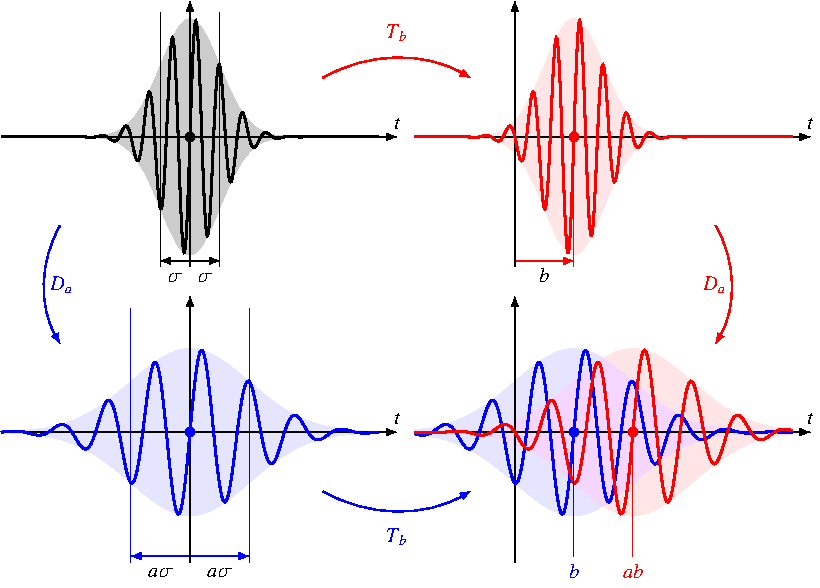
\includegraphics{chapters/2-fourier/images/kommutatorD.pdf}
\caption{Vertauschungsregel für die Operationen $T_b$ und $D_a$
(vergleiche auch Abbildung~\ref{geometrie:kommutator:image} für
die Operationen $T_b$ und $\tilde{D}_a$).
Die Graphen der Bildfunktionen unter $D_a$ sind gegenüber denen der
Bildfunktionen von $\tilde{D}_a$ vertikal um den Faktor $\sqrt{a}$
gestaucht.
\label{geometrie:kommutatorD:image}}
\end{figure}

Die Vertauschungsregel für $T_b$ und $D_a$ ist in
Abbildung~\ref{geometrie:kommutatorD:image} visualisiert.
\index{Vertauschungsregel}%

Satz~\ref{fourier:satz:TDisometrie} zeigt, dass die Operatoren $T_b$
und $D_a$ Isometrien sind.
Aus den Formeln~\eqref{fourier:satz:formel:isometrie} lässt sich aber
noch mehr schliessen.
Für zwei beliebige Funktionen $f,g\in L^2$ gilt nämlich
\begin{align*}
\langle T_af,g\rangle
&=
\langle T_{-a}T_af,T_{-a}g\rangle
=
\langle f,T_{-a}g\rangle
\\
\langle D_af,g\rangle
&=
\langle D_{1/a}D_af,D_{1/a}g\rangle
=
\langle f,D_{1/a}g\rangle.
\end{align*}
Der zu einem Operator $A$ auf einem Hilbertraum $H$ adjungierte Operatore
\index{adjungiert}%
$A^*$ ist definiert durch die Eigenschaft, dass
\[
\langle Ax,y\rangle = \langle x,A^*y\rangle
\qquad
\forall x,y\in H.
\]
Die Existenz eines adjungierten Operators folgt aus dem Darstellungssatz
von Riesz, Satz \ref{geometrie:satz:riesz}.
Für reelle Matrizen ist der adjungierte Operator die transponierte Matrix.
Mit obiger Rechnung haben wir die adjungierten Operatoren von $T_b$ und $D_a$
gefunden.

\begin{satz}
\label{fourier:satz:adjungierte}
Die adjungierten Operatoren von $T_b$ und $D_a$ sind
$T_b^* = T_{-b}$ und $D_a^*=D_{1/a}$.
\end{satz}



